\documentclass{article}
\usepackage[utf8]{inputenc}
\usepackage[export]{adjustbox}
\usepackage{wrapfig}
\usepackage{graphicx}

\title{What You Need to Know About Augmented and Virtual Reality: A CRDDS Guide}
\author{Julia Uhr}
\date{May 2020}

\begin{document}

\maketitle
\tableofcontents

\section{Introduction}
This document is intended to help CRDDS employees familiarize themselves with AR/VR technology and advise students and faculty working on AR/VR projects.

\section{Terminology}
\subsection{Augmented Reality}
Augmented reality (AR) superimposes digital elements on the real world. Currently, AR usually involves viewing the real world through the camera on a phone or tablet, but it can also involve projected images or head-mounted displays.From the developer's perspective, AR applications generally fall into three categories depending on how the app determines where to place digital objects.\\

\begin{wrapfigure}{R}{.35\textwidth}
\centering

\includegraphics[width=.3\textwidth]{hiro}
\caption{AR marker}
\end{wrapfigure}

\subsubsection{Marker-Based} Marker-based AR apps use predetermined, often barcode-like images (Figure 1) placed in the physical world to determine the location of digital objects. This is the simplest form of AR to implement.\\

\subsubsection{Location-Based} Location-based AR apps use maps and GPS coordinates to place digital objects in specific geographical locations. Examples include Pokemon-Go and Minecraft Earth.\\

\begin{wrapfigure}{R}{.6\textwidth}
\centering
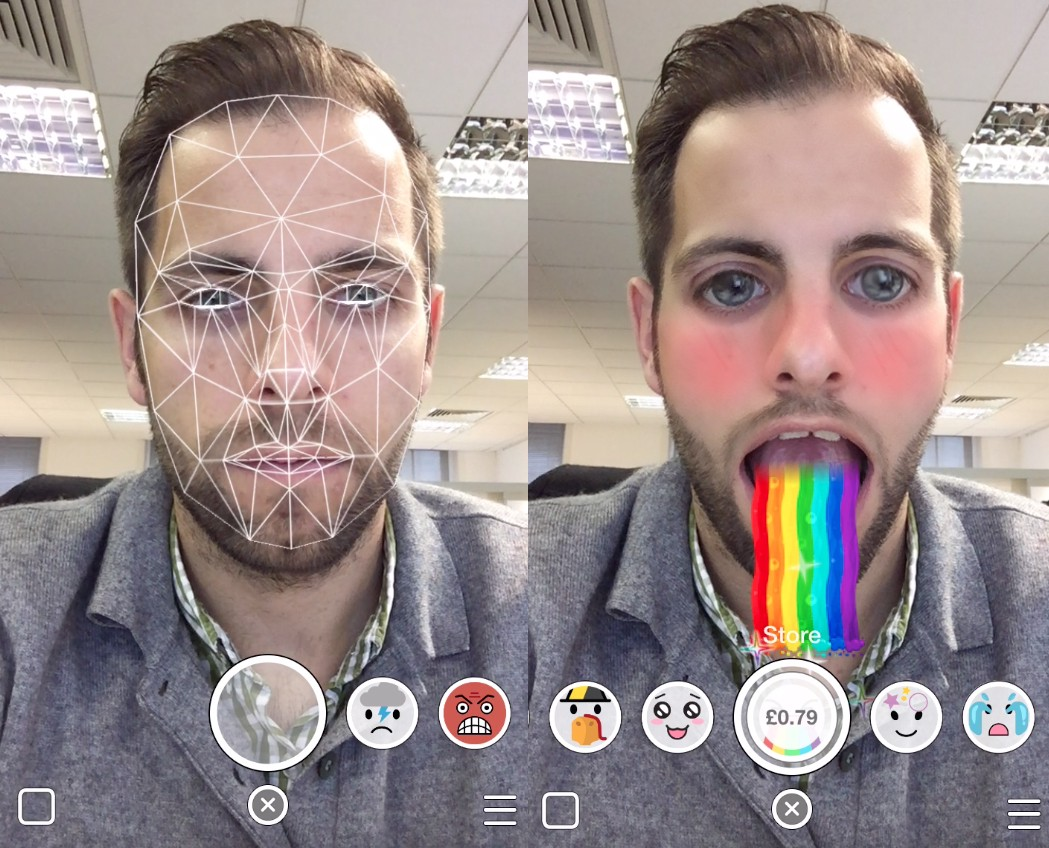
\includegraphics[width=.55\textwidth]{snap}
\caption{Snap Chat filter}
\end{wrapfigure}

\subsubsection{Image-based} Image-based, or markerless, AR apps use real-time image tracking to determine where to place digital objects or effects. This is the most complicated type of AR to implement. Examples include Snap Chat filters (Figure 2), hand-tracking applications, and Zoom backgrounds.

\subsection{Virtual Reality}

Virtual Reality (VR) uses head-mounted displays to immerse the user in a completely digital world.

\subsubsection{Head-Mounted Displays} Head-mounted displays (HMDs) are headsets that display stereo images in front of the user's eyes. By displaying different images in front of each eye, the HMD creates the appearance of a 3D image, and by tracking the movement of the user's head, it changes the images displayed to match the user's changing perspective. This creates a realistic impression of looking around inside of a 3D environment.

\subsubsection{PC VR} PC VR headsets connect via cable to a computer, like the Valve Index, the Oculus Rift, and the HTC Vive. Sometimes PC VR headsets also use external cameras placed around the room for movement-tracking. Using a PC VR headset with a powerful gaming PC can produce the most complex and realistic VR experiences currently available to consumers. However, they are not portable, and the user's movements are constrained by the length of the cables connecting the headset to the computer.

\subsubsection{Mobile VR} Mobile VR headsets do not need to connect to a PC. They are either standalone headsets, which contain all necessary computing hardware inside the headset (like the Oculus Quest), or they use a smartphone to do the computing and display (like the Google Cardboard). Mobile VR is more portable than PC VR and is not constrained by cables, but it is not powerful enough to run the most complex VR applications. Performance is a very important consideration for mobile VR developers.

\begin{wrapfigure}{R}{.6\textwidth}
\centering
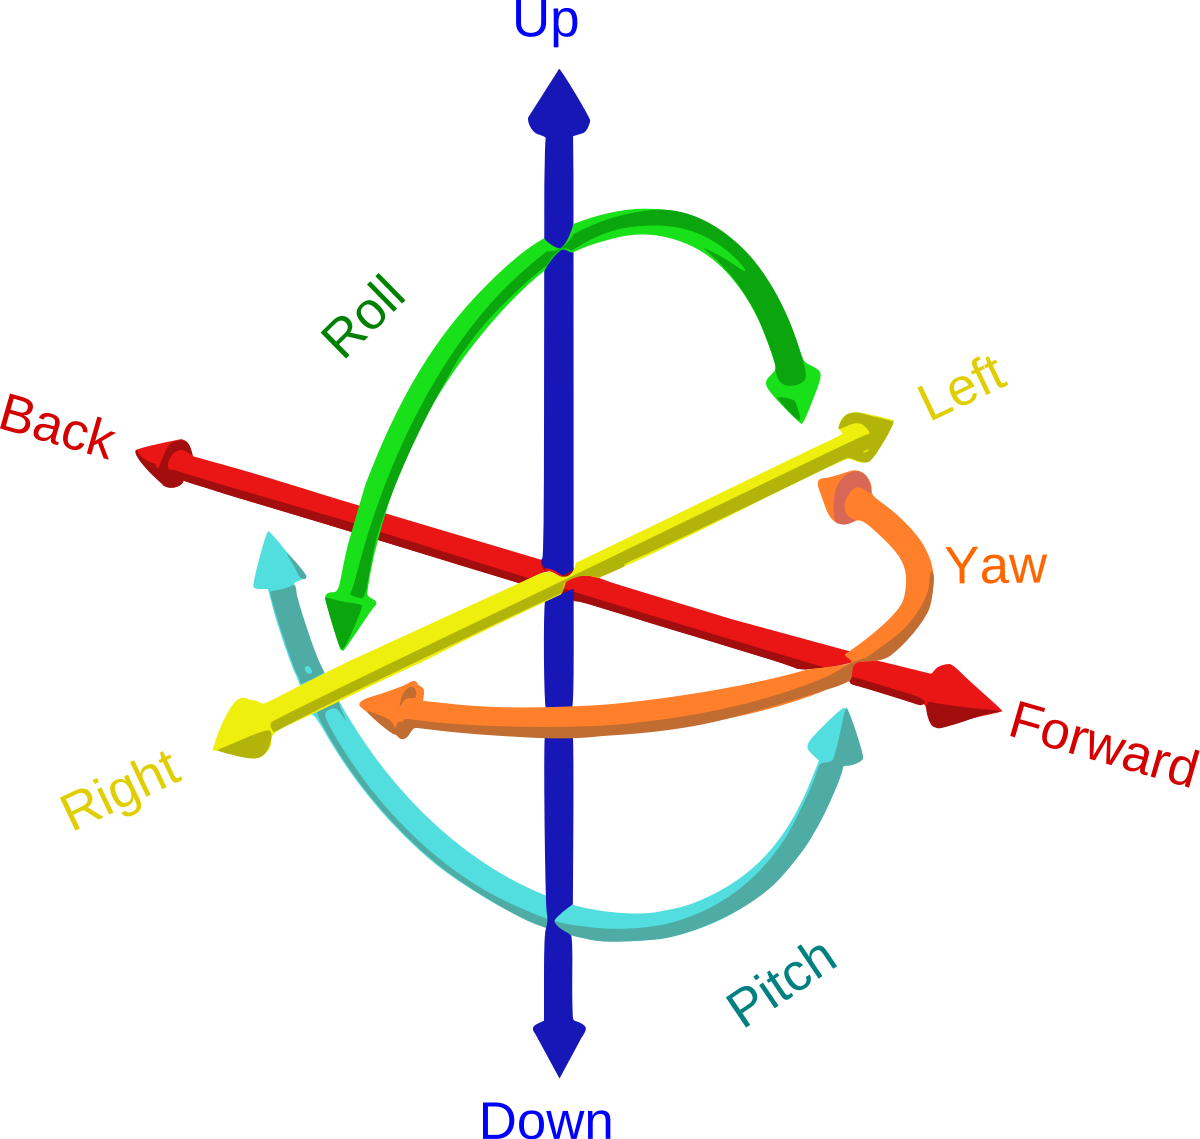
\includegraphics[width=.55\textwidth]{dof}
\caption{The six degrees of freedom}
\end{wrapfigure}

\subsubsection{Degrees of Freedom} Degrees of freedom (DoF) measure the amount of movement-tracking possible with an HMD and the controllers (if any) that go with it. 3DoF headsets can track the rotation of the user's head (and hands) as it tilts up and down, tilts side to side, and turns right and left. 6DoF headsets, in addition to tracking the three degrees of rotation, can also track the user's movements forward, backward, up, down, and side to side (Figure 3). 6DoF enables interactions like reaching out to touch an object, or walking over to something to look at it more closely. Currently, PC VR tends to have 6DoF, while mobile VR tends to have 3DoF. However, there are exceptions, and newer headsets tend to have 6DoF because it enables more realistic interactions and room-scale VR. 

\subsubsection{Room-Scale} Room-scale VR is the combination of 6DoF hardware tracking and software designed for the user to move through the virtual world by physically walking around, which increases the user's sense of immersion.

\subsection{Mixed Reality}

Mixed reality (MR) is a somewhat nebulous term that can refer to anything on the AR-VR spectrum, hardware that can display both AR and VR, or videos that combine green screen footage of a person wearing a VR headset with footage of the VR experience they're interacting with, so the video shows a real person interacting with a virtual environment.

\begin{wrapfigure}{R}{.7\textwidth}
\centering
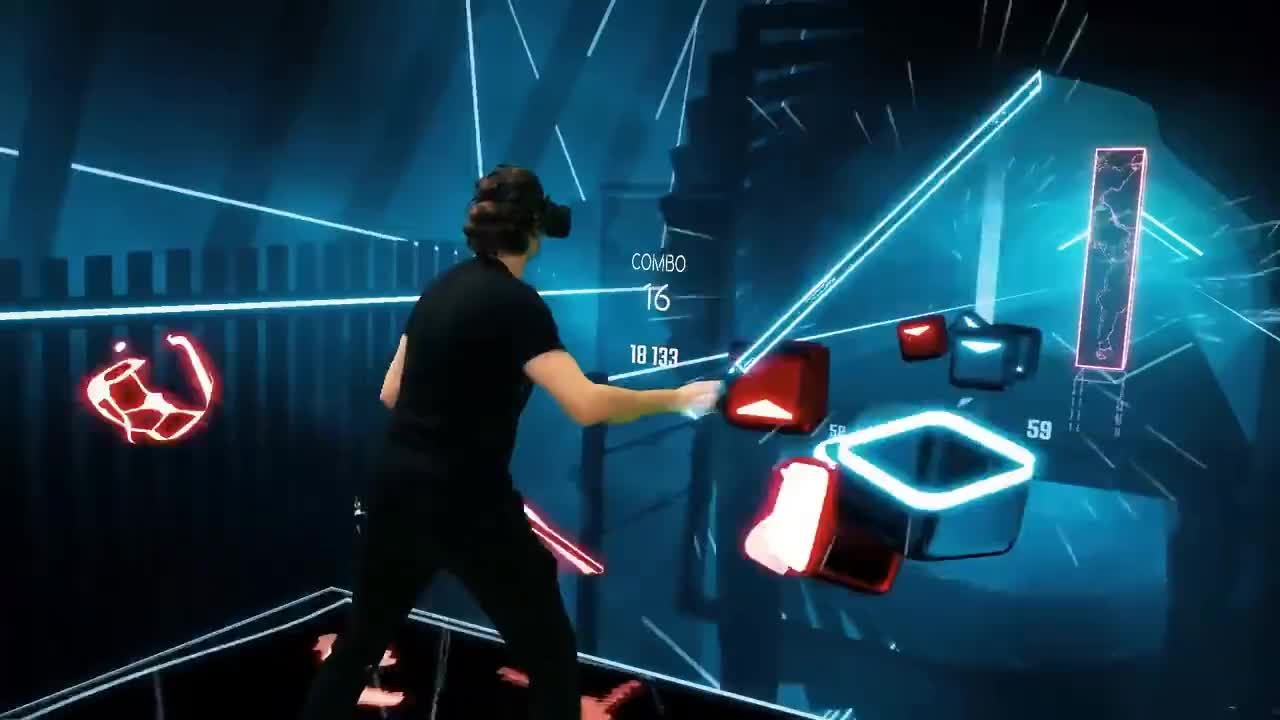
\includegraphics[width=.6\textwidth]{beatsaber}
\caption{MR Beat Saber footage}
\end{wrapfigure}

\subsection{XR (Extended Reality)}
XR is a blanket term for experiences that add digital elements to the world. It includes AR, VR, mixed reality, and any yet-to-be-invented methods of combining the physical and digital worlds.

\section{Hardware and Headsets}
There are many different headsets available. The main factors to consider when choosing which one to buy are specs, portability, and price. Also keep in mind that AR and VR technology is changing quickly. The equipment you buy will likely be out of date in a couple of years. However, as AR and VR technology progresses, prices will continue to drop an quality will continue to rise.

\begin{wrapfigure}{R}{.65\textwidth}
\centering
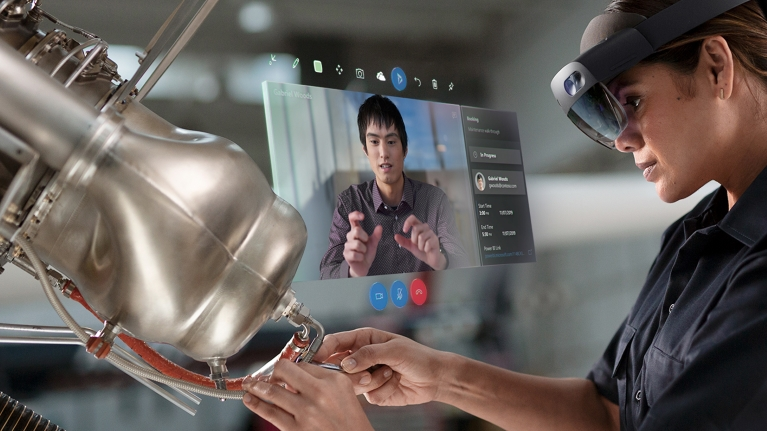
\includegraphics[width=.6\textwidth]{hololens}
\caption{Microsoft HoloLens}
\end{wrapfigure}

\subsection{AR Hardware}
Currently, most AR apps are designed to run on mobile devices, include most recent smart phones and tablets. There are also some AR headsets available that display digital images on transparent lenses. These headsets cost around 2000 to 3000 dollars and are intend mostly for enterprise, rather than consumer, uses:
\begin{itemize}
    \item Google Glass Enterprise Edition 2\\
    https://www.google.com/glass/start
    \item Microsoft HoloLens 2\\
    https://www.microsoft.com/en-us/hololens
    \item Magic Leap 1\\
    https://www.magicleap.com/en-us
\end{itemize}

\subsection{VR Hardware}
Unlike AR, VR requires a headset, but there are a wide range of headsets available. When choosing a VR headset, first consider what you want to use it for. Do you want to run large point-cloud data visualizations? If so, you probably want a PC VR headset. Do you want a headset that can travel to conferences with you? Then you probably want a mobile VR headset. Also consider how much money you want to spend and what equipment you already have. Do you have a high-end gaming PC? If not, buying one will be an additional cost of using PC VR. Do you have a new smart phone? If you do, you can get started with VR easily using a cheap phone-based headset. Here are some popular VR headsets and their approximate prices:

\begin{itemize}
    \item Google Cardboard, \$10, phone required\\
    Google no longer makes these, but copies are widely available.
    \item Samsung Gear VR, \$60, phone required\\
    https://www.samsung.com/global/galaxy/gear-vr
    \item Oculus Go, \$150, standalone\\
    https://www.oculus.com/go
    \item Oculus Quest, \$400, standalone, can run PC apps with link cable\\
    https://www.oculus.com/quest
    \item Oculus Rift-S, PC required\\
    https://www.oculus.com/rift-s
    \item Vive Cosmos, \$700, PC required\\
    https://www.vive.com/us/product/\#cosmos\%20series
    \item Valve Index, \$1000 PC required\\
    https://store.steampowered.com/valveindex
    \item Vive Pro, \$1,200, PC required\\
    https://www.vive.com/us/product/\#pro\%20series
\end{itemize}

\section{Software Tools}
This section will Developing AR and VR applications.
For simple projects and beginner developers, A-Frame and AR.js are a good place to start. For developers wanting to make more high-end applications, it is worth learning Unreal Engine or Unity.

\subsection{A-Frame}
A-Frame is an open source framework for building VR scenes that run in the web browser. A-Frame's simple, HTML-like markup language make it easy to get started with, and it can be easily extended using its component system. A-Frame scenes work both in VR and in regular 3D. A-Frame can also be used in conjunction with AR.js to make AR apps. The A-Frame source code is at https://github.com/aframevr/aframe.

\subsection{AR.js}
AR.js is an open source library for making web-based AR apps. It can make marker-based, location-based, and image-tracking AR. It works with A-Frame, using the same simple markup language. The AR.js source code is at https://github.com/AR-js-org/AR.js.

\begin{wrapfigure}{R}{.5\textwidth}
\centering
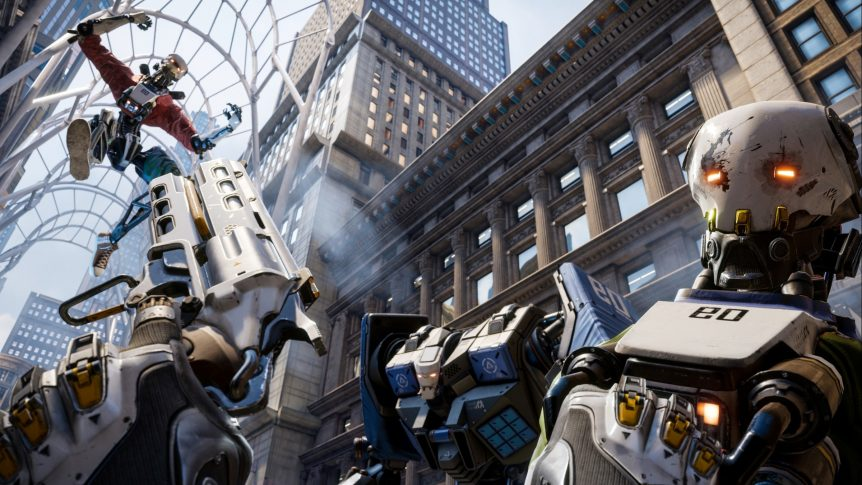
\includegraphics[width=.45\textwidth]{robo}
\caption{Robo Recall, a VR game made with Unreal}
\end{wrapfigure}

\subsection{Game Engines}
The popular game engines, Unreal (https://www.unrealengine.com) and Unity (https://unity.com), both make AR and VR development easier. These are complicated pieces of software with a steep learning curve, but they are capable of creating polished applications with high-end graphics, and they have ample resources for learning the software. Unreal Engine is free but charges royalties on monetized applications that receive revenue exceeding \$1,000,000. Unity has a free version with fewer features and charges \$40 or \$150 per month for versions with more features.

\section{Educational Resources}

\subsection{A-Frame and AR.js Tutorials}
\begin{itemize}
    \item CRDDS A-Frame AR Tutorial\\
    cu-boulder-crdds.github.io/LearningMaterials/AR.html
    \item Get Started with AR.js\\
    https://dev.to/aschmelyun/so-you-want-to-get-started-with-ar-js-22e2
    \item Build your Location-Based Augmented Reality Web App\\
    medium.com/chialab-open-source/build-your-location-based-augmented-reality-web-app-c2442e716564
    \item CRDDS A-Frame VR Tutorial\\
    cu-boulder-crdds.github.io/LearningMaterials/vr.html
    \item A-Frame School\\
    aframe.io/aframe-school/\#/
    \item VR Endless Runner\\
    smashingmagazine.com/2019/03/virtual-reality-endless-runner-game-vr-part-1/
\end{itemize}

\subsection{Game Engine Resources}

\textbf{Unreal Engine's online courses}\\
www.unrealengine.com/en-US/onlinelearning-course\\
\\
\textbf{Unreal Engine's VR resources}\\
docs.unrealengine.com/en-US/Platforms/VR/index.html\\
\\
\textbf{Unreal Engine's AR resources}\\
docs.unrealengine.com/en-US/Platforms/AR/HandheldAR/AROverview/index.html
\\
\begin{wrapfigure}{R}{.6\textwidth}
\centering
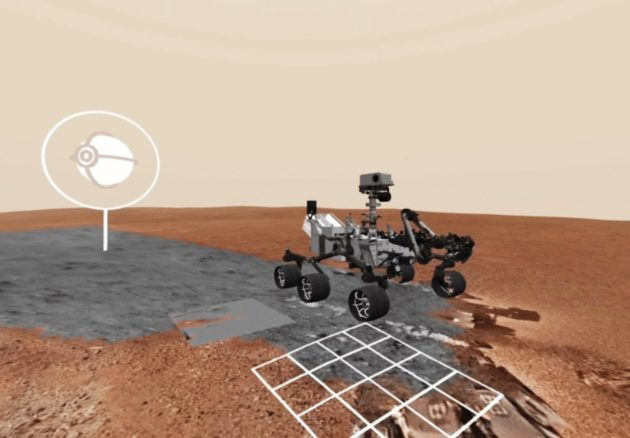
\includegraphics[width=.55\textwidth]{mars}
\caption{Access Mars}
\end{wrapfigure}
\\
\textbf{Unity's online courses}\\
learn.unity.com/\\
\\
\textbf{Unity's VR resources}\\
learn.unity.com/course/oculus-vr\\
\\
\textbf{Unity's AR resources}\\
unity.com/unity/features/ar

\subsection{AR/VR News}
roadtovr.com\\
uploadvr.com\\
vrscout.com\\

\subsection{Inspiration}

\textbf{Dance Tonite VR music video}\\
tonite.dance\\
\\
\textbf{Access Mars VR educational experience}\\
accessmars.withgoogle.com\\
\\
\textbf{Moon Rider VR rhythm game}\\
moonrider.xyz\\
\\
\textbf{Night Sky VR planetarium with real-time astronomical data}\\
supermedium.com/nightsky



\end{document}
